%%%%%%%%%%%%%%%%%%%%%%%%%%%%%%%%%%%%%%%%%%%%%%%%%%%%%%%%%%%%%%%%%%%%%%%%%%%%%%%
% INFERENCE
%%%%%%%%%%%%%%%%%%%%%%%%%%%%%%%%%%%%%%%%%%%%%%%%%%%%%%%%%%%%%%%%%%%%%%%%%%%%%%%

%%%%%%%%%%%%%%%%%%% 
% INFERENCE IS SEARCH
%%%%%%%%%%%%%%%%%%%
\begin{frame}{Natural Logic Inference is Search}
  \begin{center}
    \teaserBlindInferenceNaturalOrder
  \end{center}
\end{frame}
\begin{frame}[noframenumbering]{Natural Logic Inference is Search}
  \begin{center}
   \teaserInference
  \end{center}
\end{frame}
\begin{frame}[noframenumbering]{Natural Logic Inference is Search}
  \begin{center}
    \teaserFullDerivation
  \end{center}
\end{frame}

\begin{frame}[noframenumbering]{Natural Logic Inference is Search}
\begin{center}
  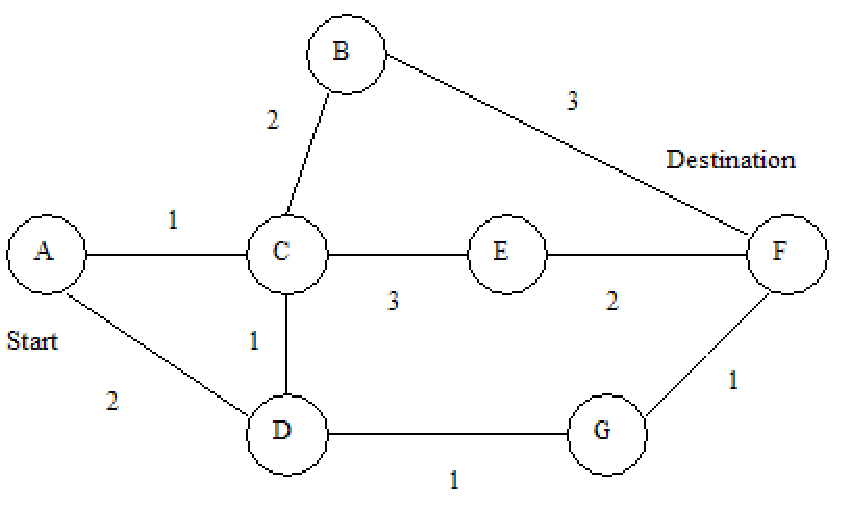
\includegraphics[width=5cm]{../../img/dijkstras-graph.pdf}
\end{center}
\begin{tabular}{ll}
  \hh{Nodes} & $($ \w{fact}, truth maintained $\in\{\textrm{true}, \textrm{false}\})$ \\
  & \\
  \pause
  \hh{Start Node} & $($ \w{query fact}, \true{true} $)$ \\
  \hh{End Nodes}  & \w{any known fact} \\
  & \\
  \pause
  \hh{Edges} & Mutations of the current fact \\
  \pause
  \hh{Edge Costs} & How ``wrong'' an inference step is (learned) \\
\end{tabular}
\end{frame}

%%%%%%%%%%%%%%%%%% 
% EXAMPLE SEARCH
%%%%%%%%%%%%%%%%%%
\input exampleSearch.tex

%%%%%%%%%%%%%%%%%%%% 
%% EDGE TEMPLATES
%%%%%%%%%%%%%%%%%%%%
%\begin{frame}{Edge Templates}
%\begin{center}
%  \begin{tabular}{p{0.4\textwidth}p{0.20\textwidth}}
%    \multicolumn{1}{c}{\textbf{Template}} & \multicolumn{1}{c}{\textbf{Instance}} \\
%    Hypernym & \w{animal} $\rightarrow$ \w{cat} \\
%    Hyponym  & \w{cat} $\rightarrow$ \w{animal} \\
%    Antonym  & \w{good} $\rightarrow$ \w{bad} \\
%    Synonym  & \w{cat} $\rightarrow$ \w{true cat} \\
%    & \\
%    Add Word  & \w{cat} $\rightarrow$ \w{$\cdot$} \\
%    Delete Word  & $\cdot$ $\rightarrow$ \w{cat} \\
%    & \\
%    Quantifier Weaken & \w{some} $\rightarrow$ \w{all} \\
%    Quantifier Strengthen & \w{all} $\rightarrow$ \w{some} \\
%    Quantifier Negate & \w{all} $\rightarrow$ \w{no} \\
%    Quantifier Synonym & \w{all} $\rightarrow$ \w{every} \\
%    & \\
%    Nearest Neighbor  & \w{cat} $\rightarrow$ \w{dog} \\
%  \end{tabular}
%\end{center}
%\end{frame}


%%%%%%%%%%%%%%%%%%%% 
%% DELETIONS (INSERTIONS)
%%%%%%%%%%%%%%%%%%%%
%\begin{frame}{Inserting Words During Search}
%\begin{center}
%  \scalebox{0.8}{\wordthe \cat \eat \mice}
%\end{center}
%\end{frame}
%
%\begin{frame}[noframenumbering]{Inserting Words During Search}
%\begin{center}
%  \scalebox{0.8}{\wordthe \cat \eat \worda \mice}
%\end{center}
%\end{frame}
%
%\def\worda{\monoUpR{}{???}{}{}}
%\begin{frame}[noframenumbering]{Inserting Words During Search}
%\begin{center}
%  \scalebox{0.8}{\wordthe \cat \eat \worda \mice} \\
%  \vspace{0.5cm}
%  \exampleInsertions
%\end{center}
%\end{frame}
%
%%%%%%%%%%%%%%%%%%%% 
%% STORE FACTS AS A TRIE
%%%%%%%%%%%%%%%%%%%%
%\def\title{Store Facts as a Trie}
%\begin{frame}{\title}
%  \factTrie{dotpath}{dotpath}{dotpath}
%\end{frame}
%
%\begin{frame}[noframenumbering]{\title}
%  \factTrie{goodPath}{dotpath}{dotpath}
%\end{frame}
%
%\begin{frame}[noframenumbering]{Inserting Words During Search}
%\begin{center}
%  \scalebox{0.8}{\wordthe \cat \eat \worda \mice}
%\end{center}
%\end{frame}
%
%\def\worda{\monoUpR{}{catnip}{herb}{tracheophyte}}
%\begin{frame}[noframenumbering]{Inserting Words During Search}
%\begin{center}
%  \scalebox{0.8}{\wordthe \cat \eat \worda \mice}
%\end{center}
%\end{frame}
%
%\begin{frame}[noframenumbering]{\title}
%  \factTrie{dotpath}{goodPath}{dotpath}
%\end{frame}
%
%\def\worda{\monoUpR{}{???}{}{}}
%\begin{frame}[noframenumbering]{Inserting Words During Search}
%\begin{center}
%  \scalebox{0.8}{\wordthe \cat \eat \worda \mice}
%\end{center}
%\end{frame}
%
%\def\worda{\monoUpR{}{my}{}{}}
%\begin{frame}[noframenumbering]{Inserting Words During Search}
%\begin{center}
%  \scalebox{0.8}{\wordthe \cat \eat \worda \mice}
%\end{center}
%\end{frame}
%
%\begin{frame}[noframenumbering]{\title}
%  \factTrie{dotpath}{dotpath}{goodPath}
%\end{frame}
%
%\def\worda{\monoUpR{}{???}{}{}}
%\begin{frame}[noframenumbering]{Inserting Words During Search}
%\begin{center}
%  \scalebox{0.8}{\wordthe \cat \eat \worda \mice}
%\end{center}
%\end{frame}
%
%\def\worda{\monoUpR{\textbf{All$_{\downarrow \uparrow}$}}{\darkgreen{\textbf{a$_{\uparrow \uparrow}$}}}{}{}}
%\begin{frame}[noframenumbering]{Inserting Words During Search}
%\begin{center}
%  \scalebox{0.8}{\wordthe \cat \eat \worda \mice}
%\end{center}
%\end{frame}

%%%%%%%%%%%%%%%%%%% 
% CONTRIBUTION: COLLAPSED INFERENCE STATES
%%%%%%%%%%%%%%%%%%%
\def\joinTable#1{
  \begin{tabular}{|c||c|c|c|c|c|c|c|}
    \hline
    $\bowtie$ & $\equivalent$ & $\forward$ & $\reverse$ & $\negate$ & $\alternate$ & $\cover$ & $\independent$ \\
    \hline
    $\equivalent$ & $\equivalent$ & $\forward$ & $\reverse$ & $\negate$ & $\alternate$ & $\cover$ & $\independent$ \\
    $\forward$ & $\forward$ & $\forward$ & $\independent$ & $\alternate$ & $\alternate$ & $\independent$ & $\independent$ \\
    $\reverse$ & $\reverse$ & $\independent$ & $\reverse$ & $\cover$ & $\independent$ & $\cover$ & $\independent$  \\
    $\negate$ & $\negate$ & $\cover$ & $\alternate$ & $\equivalent$ & $\reverse$ & $\forward$ & $\independent$  \\
    $\alternate$ & $\alternate$ & $\independent$ & $\alternate$ & \textcolor<#1-#1>{darkred}{$\forward$} & $\independent$ & $\forward$ & $\independent$  \\
    $\cover$ & $\cover$ & $\cover$ & $\independent$ & $\reverse$ & $\reverse$ & $\independent$ & $\independent$  \\
    $\independent$ & $\independent$ & $\independent$ & $\independent$ & $\independent$ & $\independent$ & $\independent$ & $\independent$ \\
    \hline
	\end{tabular}
}

\def\title{Contribution: Simple Transitivity}
\begin{frame}{\title}

  \hh{Taken for granted:} $A \Rightarrow B$ and $B \Rightarrow C$ then $A \Rightarrow C$. \\
  \vspace{0.5cm}
  \pause
  \hh{More complicated in (prior work on) Natural Logic:}
  \begin{itemize}
    \item 
      \w{nocturnal} $\xrightarrow{\alternate}$ \w{diurnal}, \hspace{0.5cm}
      \w{all} $\xrightarrow{\negate}$ \w{not all} \\
      $\therefore$  \hspace{0.1cm}
      \w{all bats are nocturnal} $\xrightarrow{?}$ \w{not all bats are diurnal}
  \end{itemize}
  \pause

  \begin{center}
    \joinTable{4}
  \end{center}
  \pause
  \pause

  \begin{textblock*}{2cm}(5.5cm,5.5cm)
    \only<5>{\scalebox{10.0}{\darkred{\xmark}}}
  \end{textblock*}
\end{frame}

\begin{frame}[noframenumbering]{\title}
  \hh{Natural Logic Analog of Transitivity:} \\
  \begin{center}
  \begin{tabular}{rll}
    \textbf{State} & \textbf{Fact} & \textbf{Mutation} \\
    $\Rightarrow$ &
            \w{all bats are nocturnal},  \hspace{0.5cm} \pause &
            (\w{nocturnal} $\xrightarrow{\alternate}$ \w{diurnal})
            \pause \\
    $\Rightarrow \lnot$ &
      \w{all bats are diurnal},  \hspace{0.5cm} \pause &
            (\w{all} $\xrightarrow{\negate}$ \w{not all})
            \pause \\
    $\Rightarrow$ &
            \w{not all bats are diurnal} &
  \end{tabular}
  \end{center}
  \pause

  \begin{itemize}
    \item Maintain correct Natural Logic inference tracking only 
          \textit{valid} and \textit{invalid} at each state.
  \end{itemize}
\end{frame}



%\def\blurb{
%\hh{Inference according to us:} The truth of a node is \textit{maintained} or
%  \textit{flipped} based on the template of the outgoing edge}
%\begin{frame}{\title}
%\blurb.
%\end{frame}
%
%\begin{frame}[noframenumbering]{\title}
%\blurb\ \darkgreen{\textbf{and the truth of the parent}}.
%\end{frame}
%
%\begin{frame}[noframenumbering]{\title}
%\blurb\ and the truth of the parent 
%  \darkgreen{\textbf{and the particular governing quantifiers}}.
%\end{frame}
%
%\def\blurb{
%\hh{Inference according to us:} The truth of a node is \textbf{\textit{maintained} or
%  \textit{flipped}} based on the template of the outgoing edge and the truth of the parent 
%  and the particular governing quantifiers.
%}
%\begin{frame}[noframenumbering]{\title}
%\blurb
%\end{frame}
%
%
%\begin{frame}[noframenumbering]{\title}
%\blurb \\
%\begin{center}	
%  \w{mammal} \reverse\ \w{cat} $~~\vdash~~$ \w{all mammals have fur} $\forward$ \w{all cats have fur} \\
%  \pause
%  \vspace{0.25cm}
%  \joinTable
%\end{center}
%\end{frame}
%
%\begin{frame}[noframenumbering]{\title}
%\blurb \\
%\begin{center}	
%  \uline{\w{mammal} \reverse\ \w{cat}} $~~\vdash~~$ \w{all mammals have fur} $\forward$ \w{all cats have fur} \\
%  \vspace{0.25cm}
%  \joinTable
%\end{center}
%\end{frame}
%
%\begin{frame}[noframenumbering]{\title}
%\blurb \\
%\begin{center}	
%  \w{mammal} \reverse\ \w{cat} $~~\vdash~~$ \uline{\w{all mammals have fur} $\forward$ \w{all cats have fur}} \\
%  \vspace{0.25cm}
%  \joinTable
%\end{center}
%\end{frame}
%
%\begin{frame}[noframenumbering]{\title}
%\blurb \\
%\begin{center}	
%  \w{mammal} \reverse\ \w{cat} $~~\vdash~~$ \uline{\w{all mammals have fur} $\Rightarrow$ \w{all cats have fur}} \\
%  \vspace{0.25cm}
%  \joinTable
%\end{center}
%\end{frame}
